% Generated by Sphinx.
\documentclass[a4paper,10pt,english]{manual}
\usepackage[utf8]{inputenc}
\usepackage[T1]{fontenc}
\usepackage{babel}
\usepackage{times}
\usepackage[Bjarne]{fncychap}
\usepackage{longtable}
\usepackage{sphinx}


\title{llCoMP Documentation}
\date{June 23, 2010}
\release{1.0}
\author{Ruymán Reyes}
\newcommand{\sphinxlogo}{}
\renewcommand{\releasename}{Release}
\makeindex
\makemodindex

\makeatletter
\def\PYG@reset{\let\PYG@it=\relax \let\PYG@bf=\relax%
    \let\PYG@ul=\relax \let\PYG@tc=\relax%
    \let\PYG@bc=\relax \let\PYG@ff=\relax}
\def\PYG@tok#1{\csname PYG@tok@#1\endcsname}
\def\PYG@toks#1+{\ifx\relax#1\empty\else%
    \PYG@tok{#1}\expandafter\PYG@toks\fi}
\def\PYG@do#1{\PYG@bc{\PYG@tc{\PYG@ul{%
    \PYG@it{\PYG@bf{\PYG@ff{#1}}}}}}}
\def\PYG#1#2{\PYG@reset\PYG@toks#1+\relax+\PYG@do{#2}}

\def\PYG@tok@gd{\def\PYG@tc##1{\textcolor[rgb]{0.63,0.00,0.00}{##1}}}
\def\PYG@tok@gu{\let\PYG@bf=\textbf\def\PYG@tc##1{\textcolor[rgb]{0.50,0.00,0.50}{##1}}}
\def\PYG@tok@gt{\def\PYG@tc##1{\textcolor[rgb]{0.00,0.25,0.82}{##1}}}
\def\PYG@tok@gs{\let\PYG@bf=\textbf}
\def\PYG@tok@gr{\def\PYG@tc##1{\textcolor[rgb]{1.00,0.00,0.00}{##1}}}
\def\PYG@tok@cm{\let\PYG@it=\textit\def\PYG@tc##1{\textcolor[rgb]{0.25,0.50,0.56}{##1}}}
\def\PYG@tok@vg{\def\PYG@tc##1{\textcolor[rgb]{0.73,0.38,0.84}{##1}}}
\def\PYG@tok@m{\def\PYG@tc##1{\textcolor[rgb]{0.13,0.50,0.31}{##1}}}
\def\PYG@tok@mh{\def\PYG@tc##1{\textcolor[rgb]{0.13,0.50,0.31}{##1}}}
\def\PYG@tok@cs{\def\PYG@tc##1{\textcolor[rgb]{0.25,0.50,0.56}{##1}}\def\PYG@bc##1{\colorbox[rgb]{1.00,0.94,0.94}{##1}}}
\def\PYG@tok@ge{\let\PYG@it=\textit}
\def\PYG@tok@vc{\def\PYG@tc##1{\textcolor[rgb]{0.73,0.38,0.84}{##1}}}
\def\PYG@tok@il{\def\PYG@tc##1{\textcolor[rgb]{0.13,0.50,0.31}{##1}}}
\def\PYG@tok@go{\def\PYG@tc##1{\textcolor[rgb]{0.19,0.19,0.19}{##1}}}
\def\PYG@tok@cp{\def\PYG@tc##1{\textcolor[rgb]{0.00,0.44,0.13}{##1}}}
\def\PYG@tok@gi{\def\PYG@tc##1{\textcolor[rgb]{0.00,0.63,0.00}{##1}}}
\def\PYG@tok@gh{\let\PYG@bf=\textbf\def\PYG@tc##1{\textcolor[rgb]{0.00,0.00,0.50}{##1}}}
\def\PYG@tok@ni{\let\PYG@bf=\textbf\def\PYG@tc##1{\textcolor[rgb]{0.84,0.33,0.22}{##1}}}
\def\PYG@tok@nl{\let\PYG@bf=\textbf\def\PYG@tc##1{\textcolor[rgb]{0.00,0.13,0.44}{##1}}}
\def\PYG@tok@nn{\let\PYG@bf=\textbf\def\PYG@tc##1{\textcolor[rgb]{0.05,0.52,0.71}{##1}}}
\def\PYG@tok@no{\def\PYG@tc##1{\textcolor[rgb]{0.38,0.68,0.84}{##1}}}
\def\PYG@tok@na{\def\PYG@tc##1{\textcolor[rgb]{0.25,0.44,0.63}{##1}}}
\def\PYG@tok@nb{\def\PYG@tc##1{\textcolor[rgb]{0.00,0.44,0.13}{##1}}}
\def\PYG@tok@nc{\let\PYG@bf=\textbf\def\PYG@tc##1{\textcolor[rgb]{0.05,0.52,0.71}{##1}}}
\def\PYG@tok@nd{\let\PYG@bf=\textbf\def\PYG@tc##1{\textcolor[rgb]{0.33,0.33,0.33}{##1}}}
\def\PYG@tok@ne{\def\PYG@tc##1{\textcolor[rgb]{0.00,0.44,0.13}{##1}}}
\def\PYG@tok@nf{\def\PYG@tc##1{\textcolor[rgb]{0.02,0.16,0.49}{##1}}}
\def\PYG@tok@si{\let\PYG@it=\textit\def\PYG@tc##1{\textcolor[rgb]{0.44,0.63,0.82}{##1}}}
\def\PYG@tok@s2{\def\PYG@tc##1{\textcolor[rgb]{0.25,0.44,0.63}{##1}}}
\def\PYG@tok@vi{\def\PYG@tc##1{\textcolor[rgb]{0.73,0.38,0.84}{##1}}}
\def\PYG@tok@nt{\let\PYG@bf=\textbf\def\PYG@tc##1{\textcolor[rgb]{0.02,0.16,0.45}{##1}}}
\def\PYG@tok@nv{\def\PYG@tc##1{\textcolor[rgb]{0.73,0.38,0.84}{##1}}}
\def\PYG@tok@s1{\def\PYG@tc##1{\textcolor[rgb]{0.25,0.44,0.63}{##1}}}
\def\PYG@tok@gp{\let\PYG@bf=\textbf\def\PYG@tc##1{\textcolor[rgb]{0.78,0.36,0.04}{##1}}}
\def\PYG@tok@sh{\def\PYG@tc##1{\textcolor[rgb]{0.25,0.44,0.63}{##1}}}
\def\PYG@tok@ow{\let\PYG@bf=\textbf\def\PYG@tc##1{\textcolor[rgb]{0.00,0.44,0.13}{##1}}}
\def\PYG@tok@sx{\def\PYG@tc##1{\textcolor[rgb]{0.78,0.36,0.04}{##1}}}
\def\PYG@tok@bp{\def\PYG@tc##1{\textcolor[rgb]{0.00,0.44,0.13}{##1}}}
\def\PYG@tok@c1{\let\PYG@it=\textit\def\PYG@tc##1{\textcolor[rgb]{0.25,0.50,0.56}{##1}}}
\def\PYG@tok@kc{\let\PYG@bf=\textbf\def\PYG@tc##1{\textcolor[rgb]{0.00,0.44,0.13}{##1}}}
\def\PYG@tok@c{\let\PYG@it=\textit\def\PYG@tc##1{\textcolor[rgb]{0.25,0.50,0.56}{##1}}}
\def\PYG@tok@mf{\def\PYG@tc##1{\textcolor[rgb]{0.13,0.50,0.31}{##1}}}
\def\PYG@tok@err{\def\PYG@bc##1{\fcolorbox[rgb]{1.00,0.00,0.00}{1,1,1}{##1}}}
\def\PYG@tok@kd{\let\PYG@bf=\textbf\def\PYG@tc##1{\textcolor[rgb]{0.00,0.44,0.13}{##1}}}
\def\PYG@tok@ss{\def\PYG@tc##1{\textcolor[rgb]{0.32,0.47,0.09}{##1}}}
\def\PYG@tok@sr{\def\PYG@tc##1{\textcolor[rgb]{0.14,0.33,0.53}{##1}}}
\def\PYG@tok@mo{\def\PYG@tc##1{\textcolor[rgb]{0.13,0.50,0.31}{##1}}}
\def\PYG@tok@mi{\def\PYG@tc##1{\textcolor[rgb]{0.13,0.50,0.31}{##1}}}
\def\PYG@tok@kn{\let\PYG@bf=\textbf\def\PYG@tc##1{\textcolor[rgb]{0.00,0.44,0.13}{##1}}}
\def\PYG@tok@o{\def\PYG@tc##1{\textcolor[rgb]{0.40,0.40,0.40}{##1}}}
\def\PYG@tok@kr{\let\PYG@bf=\textbf\def\PYG@tc##1{\textcolor[rgb]{0.00,0.44,0.13}{##1}}}
\def\PYG@tok@s{\def\PYG@tc##1{\textcolor[rgb]{0.25,0.44,0.63}{##1}}}
\def\PYG@tok@kp{\def\PYG@tc##1{\textcolor[rgb]{0.00,0.44,0.13}{##1}}}
\def\PYG@tok@w{\def\PYG@tc##1{\textcolor[rgb]{0.73,0.73,0.73}{##1}}}
\def\PYG@tok@kt{\def\PYG@tc##1{\textcolor[rgb]{0.56,0.13,0.00}{##1}}}
\def\PYG@tok@sc{\def\PYG@tc##1{\textcolor[rgb]{0.25,0.44,0.63}{##1}}}
\def\PYG@tok@sb{\def\PYG@tc##1{\textcolor[rgb]{0.25,0.44,0.63}{##1}}}
\def\PYG@tok@k{\let\PYG@bf=\textbf\def\PYG@tc##1{\textcolor[rgb]{0.00,0.44,0.13}{##1}}}
\def\PYG@tok@se{\let\PYG@bf=\textbf\def\PYG@tc##1{\textcolor[rgb]{0.25,0.44,0.63}{##1}}}
\def\PYG@tok@sd{\let\PYG@it=\textit\def\PYG@tc##1{\textcolor[rgb]{0.25,0.44,0.63}{##1}}}

\def\PYGZbs{\char`\\}
\def\PYGZus{\char`\_}
\def\PYGZob{\char`\{}
\def\PYGZcb{\char`\}}
\def\PYGZca{\char`\^}
% for compatibility with earlier versions
\def\PYGZat{@}
\def\PYGZlb{[}
\def\PYGZrb{]}
\makeatother

\begin{document}

\maketitle
\tableofcontents
\hypertarget{--doc-index}{}


llCoMP is a translator framework designed for \emph{fast prototyping}.
With little effort, you can build translators from OpenMP/C to different High
Performance Computing languages, libraries and frameworks.  Currently we have
implemented the CUDA Backend, but we have plans to implement new ones.
\hypertarget{layered-design}{}\begin{figure}[htbp]
\centering

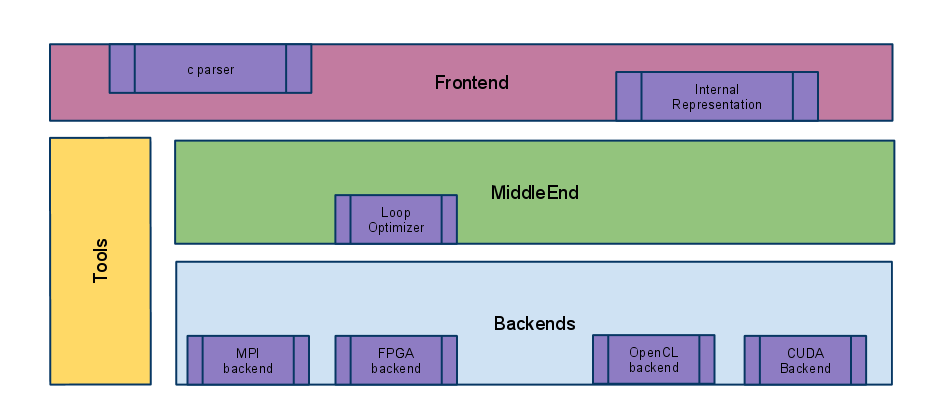
\includegraphics{layered_design.png}
\end{figure}

In the diagram (layered\_design), the different layers of the framework are exposed.

The uppermost level contains the \hyperlink{module-Frontend}{\code{Frontend}}, which gives the tools required to transform
the source code into the internal representation.

The \code{MiddleEnd} module encapsulates transformations from the IR to the IR, for example,
loop optimizations or type data conversions.

Finally \hyperlink{module-Backends}{\code{Backends}} module contains all the implemented backends

Tools to manipulate the internal representation (and do some other stuff), are packaged
on the \hyperlink{module-Tools}{\code{Tools}} module.

In addition, some utils and examples are presented in order to show the capabilities of the framework.

Contents:

\resetcurrentobjects
\hypertarget{--doc-frontend}{}

\chapter{Frontend}
\index{Frontend (module)}
\hypertarget{module-Frontend}{}
\declaremodule[Frontend]{}{Frontend}
\modulesynopsis{Methods to build the IR of a source file}
The frontend module builds the internal representation from a source file.

Two modules, representing the two phases of the code parsing, are written.


\section{Parsing Tools}


\section{Internal Representation}

\resetcurrentobjects
\hypertarget{--doc-backends}{}

\chapter{Backends}
\index{Backends (module)}
\hypertarget{module-Backends}{}
\declaremodule[Backends]{}{Backends}
\modulesynopsis{Repository of implemented backends}
The \hyperlink{module-Backends}{\code{Backends}} module packages the different backends implemented on the compiler.

The \hyperlink{module-Common}{\code{Common}} module contains common classes for all backends.

The \hyperlink{module-DotBackend}{\code{DotBackend}} module is able to translate the \emph{Internal
Representation} (IR) to \emph{Dot language}, which may be printed with
graphviz.

The \hyperlink{module-CBackend}{\code{CBackend}} module contains writers capable of converting the IR to
C or OpenMP code.

Module \hyperlink{module-CudaBackend}{\code{CudaBackend}} encapsulates Mutators, Visitors and Writers, capable of
translating the IR to CUDA code.

\resetcurrentobjects
\hypertarget{--doc-common}{}

\section{Common}
\index{Common (module)}
\hypertarget{module-Common}{}
\declaremodule[Common]{}{Common}
\modulesynopsis{Common classes for all backends}
The Common module contains common operations to the different backends.


\subsection{Mutators}

Some \hyperlink{term-mutator}{\emph{Mutator}} are declared on the \code{Mutators} module.


\subsubsection{AbstractMutator}

As you may see on the diagram, all mutators inherits from \code{AbstractMutator}.
\begin{figure}[htbp]
\centering

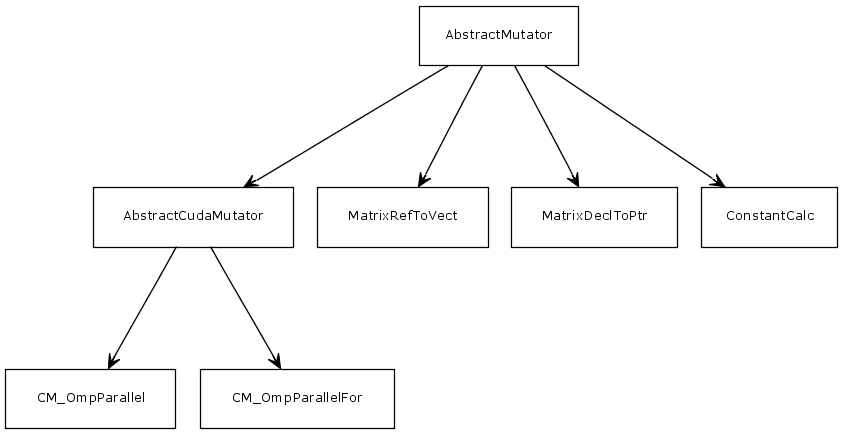
\includegraphics{mutator_inheritance.png}
\end{figure}
\index{Backends.Common.Mutators.AbstractMutator (module)}
\hypertarget{module-Backends.Common.Mutators.AbstractMutator}{}
\declaremodule[Backends.Common.Mutators.AbstractMutator]{}{Backends.Common.Mutators.AbstractMutator}
\modulesynopsis{}\index{AbstractMutator (class in Backends.Common.Mutators.AbstractMutator)}

\hypertarget{Backends.Common.Mutators.AbstractMutator.AbstractMutator}{}\begin{classdesc}{AbstractMutator}{}
Abstract class representing a mutation.
\index{apply() (Backends.Common.Mutators.AbstractMutator.AbstractMutator method)}

\hypertarget{Backends.Common.Mutators.AbstractMutator.AbstractMutator.apply}{}\begin{methoddesc}{apply}{ast, mutator\_opt\_arg=None}
Apply a mutation
\begin{quote}\begin{description}
\item[Returns] \leavevmode
filtered node

\end{description}\end{quote}
\end{methoddesc}
\index{apply\_all() (Backends.Common.Mutators.AbstractMutator.AbstractMutator method)}

\hypertarget{Backends.Common.Mutators.AbstractMutator.AbstractMutator.apply\_all}{}\begin{methoddesc}{apply\_all}{ast, mutator\_opt\_arg=None}
Apply mutation to all matches
\begin{quote}\begin{description}
\item[Returns] \leavevmode
pointer to last applied mutation

\end{description}\end{quote}
\end{methoddesc}
\index{fast\_apply\_all() (Backends.Common.Mutators.AbstractMutator.AbstractMutator method)}

\hypertarget{Backends.Common.Mutators.AbstractMutator.AbstractMutator.fast\_apply\_all}{}\begin{methoddesc}{fast\_apply\_all}{ast}
Apply mutation to all matches ignoring syntactic order
\begin{quote}\begin{description}
\item[Returns] \leavevmode
pointer to last applied mutation

\end{description}\end{quote}
\end{methoddesc}
\index{filter() (Backends.Common.Mutators.AbstractMutator.AbstractMutator method)}

\hypertarget{Backends.Common.Mutators.AbstractMutator.AbstractMutator.filter}{}\begin{methoddesc}{filter}{ast}
Calls to a simple filter
\end{methoddesc}
\index{filter\_iterator() (Backends.Common.Mutators.AbstractMutator.AbstractMutator method)}

\hypertarget{Backends.Common.Mutators.AbstractMutator.AbstractMutator.filter\_iterator}{}\begin{methoddesc}{filter\_iterator}{ast}
Calls an iterable filter
\end{methoddesc}
\index{mutatorFunction() (Backends.Common.Mutators.AbstractMutator.AbstractMutator method)}

\hypertarget{Backends.Common.Mutators.AbstractMutator.AbstractMutator.mutatorFunction}{}\begin{methoddesc}{mutatorFunction}{ast}
Mutates the AST
\begin{quote}\begin{description}
\item[Returns] \leavevmode
Starting point of the mutation

\end{description}\end{quote}
\end{methoddesc}
\end{classdesc}


\subsubsection{AstSupport}

Additional mutators are provided in order to easier the backend writing process.
\index{Backends.Common.Mutators.AstSupport (module)}
\hypertarget{module-Backends.Common.Mutators.AstSupport}{}
\declaremodule[Backends.Common.Mutators.AstSupport]{}{Backends.Common.Mutators.AstSupport}
\modulesynopsis{}\index{DeclsToParamsMutator (class in Backends.Common.Mutators.AstSupport)}

\hypertarget{Backends.Common.Mutators.AstSupport.DeclsToParamsMutator}{}\begin{classdesc}{DeclsToParamsMutator}{}
DeclsToParams
\index{convert() (Backends.Common.Mutators.AstSupport.DeclsToParamsMutator method)}

\hypertarget{Backends.Common.Mutators.AstSupport.DeclsToParamsMutator.convert}{}\begin{methoddesc}{convert}{node}
Transform a type declaration to a parameter declaration
\end{methoddesc}
\index{filter() (Backends.Common.Mutators.AstSupport.DeclsToParamsMutator method)}

\hypertarget{Backends.Common.Mutators.AstSupport.DeclsToParamsMutator.filter}{}\begin{methoddesc}{filter}{ast}
Filter definition
Returns the first node matching with the filter
\end{methoddesc}
\index{mutatorFunction() (Backends.Common.Mutators.AstSupport.DeclsToParamsMutator method)}

\hypertarget{Backends.Common.Mutators.AstSupport.DeclsToParamsMutator.mutatorFunction}{}\begin{methoddesc}{mutatorFunction}{ast}
Mutator code
\end{methoddesc}
\end{classdesc}
\index{FuncToDeviceMutator (class in Backends.Common.Mutators.AstSupport)}

\hypertarget{Backends.Common.Mutators.AstSupport.FuncToDeviceMutator}{}\begin{classdesc}{FuncToDeviceMutator}{func\_call}
Replace the definition of a FuncCall with a CUDAKernel with type \_\_device\_\_
\index{filter() (Backends.Common.Mutators.AstSupport.FuncToDeviceMutator method)}

\hypertarget{Backends.Common.Mutators.AstSupport.FuncToDeviceMutator.filter}{}\begin{methoddesc}{filter}{ast}
Find the declaration of the
\end{methoddesc}
\end{classdesc}
\index{IDNameMutator (class in Backends.Common.Mutators.AstSupport)}

\hypertarget{Backends.Common.Mutators.AstSupport.IDNameMutator}{}\begin{classdesc}{IDNameMutator}{old, new}
Replace and ID name with another ID name
\end{classdesc}
\index{RemoveAttributeMutator (class in Backends.Common.Mutators.AstSupport)}

\hypertarget{Backends.Common.Mutators.AstSupport.RemoveAttributeMutator}{}\begin{classdesc}{RemoveAttributeMutator}{attr}
Remove the child of the first apperance of an attribute inside a node
\index{apply() (Backends.Common.Mutators.AstSupport.RemoveAttributeMutator method)}

\hypertarget{Backends.Common.Mutators.AstSupport.RemoveAttributeMutator.apply}{}\begin{methoddesc}{apply}{ast}
Apply the mutation
\end{methoddesc}
\end{classdesc}


\subsection{Filter visitors}

\begin{notice}{warning}{Warning:}
Mabye a name change is needed, \emph{SearchVisitor} will be more clear.
\end{notice}

\begin{notice}{warning}{Warning:}
Some cleaning needs to be done in this module.
\end{notice}

In order to search nodes on the AST, the programmer needs to implements a \hyperlink{term-filter}{\emph{Filter}}.
\code{GenericFilterVisitor} is the parent of all filters, defining the commom methods
of all filters.

This module has other members, which are concrete implementations of the \code{GenericFilterVisitor}.
\index{Backends.Common.Visitors.GenericVisitors (module)}
\hypertarget{module-Backends.Common.Visitors.GenericVisitors}{}
\declaremodule[Backends.Common.Visitors.GenericVisitors]{}{Backends.Common.Visitors.GenericVisitors}
\modulesynopsis{}\index{GenericFilterVisitor (class in Backends.Common.Visitors.GenericVisitors)}

\hypertarget{Backends.Common.Visitors.GenericVisitors.GenericFilterVisitor}{}\begin{classdesc}{GenericFilterVisitor}{condition\_func, prev\_brother=None}
Returns the first node validating a condition function
\index{apply() (Backends.Common.Visitors.GenericVisitors.GenericFilterVisitor method)}

\hypertarget{Backends.Common.Visitors.GenericVisitors.GenericFilterVisitor.apply}{}\begin{methoddesc}{apply}{ast, ignore=, {[}{]}}
Searchs the node matching the condition\_func in the AST
\begin{quote}\begin{description}
\item[Parameters] \leavevmode\begin{itemize}
\item {} 
\emph{ast} -- Node to start search

\item {} 
\emph{ignore} -- List of nodes to ignore

\end{itemize}

\item[Returns] \leavevmode
First matching node not in ignore list

\end{description}\end{quote}
\end{methoddesc}
\index{dfs\_iter() (Backends.Common.Visitors.GenericVisitors.GenericFilterVisitor method)}

\hypertarget{Backends.Common.Visitors.GenericVisitors.GenericFilterVisitor.dfs\_iter}{}\begin{methoddesc}{dfs\_iter}{root, visited=None}
Given a starting node, root, do a depth-first search. 
.. warning:

\begin{Verbatim}[commandchars=@\[\]]
This method does not garantee to transverse the tree on the gramatically correct order
\end{Verbatim}
\begin{quote}\begin{description}
\item[Returns] \leavevmode
Last match or raise StopIteration

\end{description}\end{quote}
\end{methoddesc}
\index{generic\_visit() (Backends.Common.Visitors.GenericVisitors.GenericFilterVisitor method)}

\hypertarget{Backends.Common.Visitors.GenericVisitors.GenericFilterVisitor.generic\_visit}{}\begin{methoddesc}{generic\_visit}{node, offset=0, ignore=, {[}{]}}
Called if no explicit visitor function exists for a 
node. Implements preorder (syntactically correct) node visit.
\begin{quote}
\begin{quote}\begin{description}
\item[param node] \leavevmode
Node being visited

\item[param prev] \leavevmode
Syntactically previous node

\item[param offset] \leavevmode
Not used

\item[param ignore] \leavevmode
List of nodes to ignore

\item[return] \leavevmode
Result of the node visit

\end{description}\end{quote}
\end{quote}
\end{methoddesc}
\index{iterate() (Backends.Common.Visitors.GenericVisitors.GenericFilterVisitor method)}

\hypertarget{Backends.Common.Visitors.GenericVisitors.GenericFilterVisitor.iterate}{}\begin{methoddesc}{iterate}{ast}
Iterate through matching nodes
\begin{quote}\begin{description}
\item[Parameter] \leavevmode
\emph{ast} -- Node to start the search

\end{description}\end{quote}
\end{methoddesc}
\index{parentOfMatch() (Backends.Common.Visitors.GenericVisitors.GenericFilterVisitor method)}

\hypertarget{Backends.Common.Visitors.GenericVisitors.GenericFilterVisitor.parentOfMatch}{}\begin{methoddesc}{parentOfMatch}{}
Parent of the node matched

\begin{notice}{note}{Note:}
This is not needed because we have a .parent attribute now
\end{notice}
\end{methoddesc}
\index{visit() (Backends.Common.Visitors.GenericVisitors.GenericFilterVisitor method)}

\hypertarget{Backends.Common.Visitors.GenericVisitors.GenericFilterVisitor.visit}{}\begin{methoddesc}{visit}{node, prev, offset=1, ignore=, {[}{]}}
Finds a way to visit a node
\begin{quote}\begin{description}
\item[Parameters] \leavevmode\begin{itemize}
\item {} 
\emph{node} -- Node to visit

\item {} 
\emph{prev} -- Syntactically previous node

\item {} 
\emph{offset} -- Not used

\item {} 
\emph{ignore} -- List of nodes to ignore

\end{itemize}

\item[Returns] \leavevmode
result of the node visit

\end{description}\end{quote}
\end{methoddesc}
\end{classdesc}

\resetcurrentobjects
\hypertarget{--doc-dotbackend}{}

\section{Dot Backend}
\index{DotBackend (module)}
\hypertarget{module-DotBackend}{}
\declaremodule[DotBackend]{}{DotBackend}
\modulesynopsis{Converts IR to Dot}
The \hyperlink{module-DotBackend}{\code{DotBackend}} module contains a \code{DotWriter}, capable of
produce Dot language code from the IR.

This backend is used in the \code{Tools.Debug} tool.

The \code{DotWriter} implements a visitor pattern.
\index{Backends.DotBackend.Writers.DotWriter (module)}
\hypertarget{module-Backends.DotBackend.Writers.DotWriter}{}
\declaremodule[Backends.DotBackend.Writers.DotWriter]{}{Backends.DotBackend.Writers.DotWriter}
\modulesynopsis{}\index{DotWriter (class in Backends.DotBackend.Writers.DotWriter)}

\hypertarget{Backends.DotBackend.Writers.DotWriter.DotWriter}{}\begin{classdesc}{DotWriter}{filename=None, highlight=None}
Generates Dot code from the IR
\index{generic\_visit() (Backends.DotBackend.Writers.DotWriter.DotWriter method)}

\hypertarget{Backends.DotBackend.Writers.DotWriter.DotWriter.generic\_visit}{}\begin{methoddesc}{generic\_visit}{node, offset=0}
Called if no explicit visitor function exists for a 
node. Implements preorder visiting of the node.
\end{methoddesc}
\index{get\_name() (Backends.DotBackend.Writers.DotWriter.DotWriter method)}

\hypertarget{Backends.DotBackend.Writers.DotWriter.DotWriter.get\_name}{}\begin{methoddesc}{get\_name}{node}
Get the name of a node

\begin{notice}{note}{Note:}
This method requires further explanation
\end{notice}
\begin{quote}\begin{description}
\item[Parameter] \leavevmode
\emph{node} -- Node to get the name

\end{description}\end{quote}
\end{methoddesc}
\index{visit() (Backends.DotBackend.Writers.DotWriter.DotWriter method)}

\hypertarget{Backends.DotBackend.Writers.DotWriter.DotWriter.visit}{}\begin{methoddesc}{visit}{node, offset=0}
Visit a node
\end{methoddesc}
\index{write\_highlights() (Backends.DotBackend.Writers.DotWriter.DotWriter method)}

\hypertarget{Backends.DotBackend.Writers.DotWriter.DotWriter.write\_highlights}{}\begin{methoddesc}{write\_highlights}{}
Write a label to highlight nodes

The nodes to highlight come from self.highlight
\end{methoddesc}
\index{write\_label() (Backends.DotBackend.Writers.DotWriter.DotWriter method)}

\hypertarget{Backends.DotBackend.Writers.DotWriter.DotWriter.write\_label}{}\begin{methoddesc}{write\_label}{node, name}
Write a label for a node
\begin{quote}\begin{description}
\item[Parameters] \leavevmode\begin{itemize}
\item {} 
\emph{node} -- Label of node

\item {} 
\emph{name} -- Name of the line

\end{itemize}

\end{description}\end{quote}
\end{methoddesc}
\index{write\_line() (Backends.DotBackend.Writers.DotWriter.DotWriter method)}

\hypertarget{Backends.DotBackend.Writers.DotWriter.DotWriter.write\_line}{}\begin{methoddesc}{write\_line}{begin, name, end}
Write a connection between two nodes
\begin{quote}\begin{description}
\item[Parameters] \leavevmode\begin{itemize}
\item {} 
\emph{begin} -- Start node

\item {} 
\emph{end} -- End node

\item {} 
\emph{name} -- Name of the line

\end{itemize}

\end{description}\end{quote}
\end{methoddesc}
\end{classdesc}

\resetcurrentobjects
\hypertarget{--doc-cbackend}{}

\section{CBackend}
\index{CBackend (module)}
\hypertarget{module-CBackend}{}
\declaremodule[CBackend]{}{CBackend}
\modulesynopsis{Converts IR to C with OpenMP extensions}
The \hyperlink{module-CBackend}{\code{CBackend}} module contains two writers, \code{CWriter} and \code{OmpWriter},
which produces \textbf{C} and \textbf{OpenMP} code

\begin{notice}{note}{Note:}
This backend is widely used on llCoMP.
\end{notice}
\index{Backends.CBackend.Writers.CWriter (module)}
\hypertarget{module-Backends.CBackend.Writers.CWriter}{}
\declaremodule[Backends.CBackend.Writers.CWriter]{}{Backends.CBackend.Writers.CWriter}
\modulesynopsis{}\index{CWriter (class in Backends.CBackend.Writers.CWriter)}

\hypertarget{Backends.CBackend.Writers.CWriter.CWriter}{}\begin{classdesc}{CWriter}{filename=None, stream=None}
A visitor which translates the IR to plain C code
\index{generic\_visit\_nodeList() (Backends.CBackend.Writers.CWriter.CWriter method)}

\hypertarget{Backends.CBackend.Writers.CWriter.CWriter.generic\_visit\_nodeList}{}\begin{methoddesc}{generic\_visit\_nodeList}{nodeList, separator, offset}
Visit a list of nodes , writing values within a separator
\end{methoddesc}
\end{classdesc}
\index{Backends.CBackend.Writers.OmpWriter (module)}
\hypertarget{module-Backends.CBackend.Writers.OmpWriter}{}
\declaremodule[Backends.CBackend.Writers.OmpWriter]{}{Backends.CBackend.Writers.OmpWriter}
\modulesynopsis{}\index{OmpWriter (class in Backends.CBackend.Writers.OmpWriter)}

\hypertarget{Backends.CBackend.Writers.OmpWriter.OmpWriter}{}\begin{classdesc}{OmpWriter}{filename=None, stream=None}
Visitor which translates the IR to C/OpenMP.
\end{classdesc}

\resetcurrentobjects
\hypertarget{--doc-cudabackend}{}

\section{CUDA Backend}
\index{CudaBackend (module)}
\hypertarget{module-CudaBackend}{}
\declaremodule[CudaBackend]{}{CudaBackend}
\modulesynopsis{Converts IR to CUDA}
The \hyperlink{module-CudaBackend}{\code{CudaBackend}} module contains a set of Mutators, Filters and Templates
which creates CUDA code from the IR.


\subsection{Filters}
\index{Backends.CudaBackend.Visitors.CM\_Visitors (module)}
\hypertarget{module-Backends.CudaBackend.Visitors.CM_Visitors}{}
\declaremodule[Backends.CudaBackend.Visitors.CMVisitors]{}{Backends.CudaBackend.Visitors.CM\_Visitors}
\modulesynopsis{}\index{OmpForFilter (class in Backends.CudaBackend.Visitors.CM\_Visitors)}

\hypertarget{Backends.CudaBackend.Visitors.CM\_Visitors.OmpForFilter}{}\begin{classdesc}{OmpForFilter}{prev\_brother=None}
Returns a OmpFor node , the parallel container and the function container
\begin{description}
\item[By defining specific visitor methods for \emph{FuncDef} and \emph{OmpParallel}, we can] \leavevmode
save the last node visited of this types. Giving the fact that the visit is
done in syntax order, the last visited node will be the previous (parent) node
of the wanted node.

\end{description}
\index{iterate() (Backends.CudaBackend.Visitors.CM\_Visitors.OmpForFilter method)}

\hypertarget{Backends.CudaBackend.Visitors.CM\_Visitors.OmpForFilter.iterate}{}\begin{methoddesc}{iterate}{ast}
Iterate through matching nodes
\end{methoddesc}
\end{classdesc}
\index{OmpParallelFilter (class in Backends.CudaBackend.Visitors.CM\_Visitors)}

\hypertarget{Backends.CudaBackend.Visitors.CM\_Visitors.OmpParallelFilter}{}\begin{classdesc}{OmpParallelFilter}{condition\_func=None, prev\_brother=None, device=None}
Returns a OmpParallel node , the parallel container and the function container
\begin{description}
\item[By defining specific visitor methods for \emph{FuncDef} and \emph{OmpParallel}, we can] \leavevmode
save the last node visited of this types. Giving the fact that the visit is
done in syntax order, the last visited node will be the previous (parent) node
of the wanted node.

\end{description}
\index{parallel\_condition() (Backends.CudaBackend.Visitors.CM\_Visitors.OmpParallelFilter method)}

\hypertarget{Backends.CudaBackend.Visitors.CM\_Visitors.OmpParallelFilter.parallel\_condition}{}\begin{methoddesc}{parallel\_condition}{node}
OmpParallel filter
\end{methoddesc}
\index{visit\_OmpTargetDevice() (Backends.CudaBackend.Visitors.CM\_Visitors.OmpParallelFilter method)}

\hypertarget{Backends.CudaBackend.Visitors.CM\_Visitors.OmpParallelFilter.visit\_OmpTargetDevice}{}\begin{methoddesc}{visit\_OmpTargetDevice}{node, prev, offset=1, ignore=, {[}{]}}
Save target device node
\end{methoddesc}
\end{classdesc}
\index{OmpParallelForFilter (class in Backends.CudaBackend.Visitors.CM\_Visitors)}

\hypertarget{Backends.CudaBackend.Visitors.CM\_Visitors.OmpParallelForFilter}{}\begin{classdesc}{OmpParallelForFilter}{prev\_brother=None, device=None}
Returns a \emph{omp parallel for} construct
\end{classdesc}
\index{OmpThreadPrivateFilter (class in Backends.CudaBackend.Visitors.CM\_Visitors)}

\hypertarget{Backends.CudaBackend.Visitors.CM\_Visitors.OmpThreadPrivateFilter}{}\begin{classdesc}{OmpThreadPrivateFilter}{prev\_brother=None}
Returns the ThreadPrivate constructs
\end{classdesc}


\subsection{Templates}

Currently, templates are held inside \code{Mutators} code.


\subsection{Mutators}

A separate Mutator have been written for each OpenMP construct.
Their parent is \code{Backends.CudaBackend.Mutators.Common}
\index{Backends.CudaBackend.Mutators.Common (module)}
\hypertarget{module-Backends.CudaBackend.Mutators.Common}{}
\declaremodule[Backends.CudaBackend.Mutators.Common]{}{Backends.CudaBackend.Mutators.Common}
\modulesynopsis{}\index{AbstractCudaMutator (class in Backends.CudaBackend.Mutators.Common)}

\hypertarget{Backends.CudaBackend.Mutators.Common.AbstractCudaMutator}{}\begin{classdesc}{AbstractCudaMutator}{clauses=None, kernel\_name='loopKernel', kernel\_prefix=''}
Common methods to work with CUDA
\index{buildDeclarations() (Backends.CudaBackend.Mutators.Common.AbstractCudaMutator method)}

\hypertarget{Backends.CudaBackend.Mutators.Common.AbstractCudaMutator.buildDeclarations}{}\begin{methoddesc}{buildDeclarations}{numThreads, reduction\_node\_list, shared\_node\_list, ast}
Builds the declaration section 
@param numThreads number of threads
@return Declarations subtree
\end{methoddesc}
\index{buildHostReduction() (Backends.CudaBackend.Mutators.Common.AbstractCudaMutator method)}

\hypertarget{Backends.CudaBackend.Mutators.Common.AbstractCudaMutator.buildHostReduction}{}\begin{methoddesc}{buildHostReduction}{reduction\_vars, ast}
Instanciate the reduction pattern

@return Compound with the reduction code
\end{methoddesc}
\index{buildKernel() (Backends.CudaBackend.Mutators.Common.AbstractCudaMutator method)}

\hypertarget{Backends.CudaBackend.Mutators.Common.AbstractCudaMutator.buildKernel}{}\begin{methoddesc}{buildKernel}{shared\_list, private\_list, reduction\_list, loop, ast}
Build CUDA Kernel code
\end{methoddesc}
\index{getThreadNum() (Backends.CudaBackend.Mutators.Common.AbstractCudaMutator method)}

\hypertarget{Backends.CudaBackend.Mutators.Common.AbstractCudaMutator.getThreadNum}{}\begin{methoddesc}{getThreadNum}{node}
Gets the maximum number of threads needed
\end{methoddesc}
\index{get\_names() (Backends.CudaBackend.Mutators.Common.AbstractCudaMutator method)}

\hypertarget{Backends.CudaBackend.Mutators.Common.AbstractCudaMutator.get\_names}{}\begin{methoddesc}{get\_names}{elem, ast}
Return a list of names for a type
\end{methoddesc}
\end{classdesc}

The following constructs have been implemented:

\textbf{OpenMP Parallel}
\index{Backends.CudaBackend.Mutators.CM\_OmpParallel (module)}
\hypertarget{module-Backends.CudaBackend.Mutators.CM_OmpParallel}{}
\declaremodule[Backends.CudaBackend.Mutators.CMOmpParallel]{}{Backends.CudaBackend.Mutators.CM\_OmpParallel}
\modulesynopsis{}
\textbf{OpenMP Parallel For}
\index{Backends.CudaBackend.Mutators.CM\_OmpParallelFor (module)}
\hypertarget{module-Backends.CudaBackend.Mutators.CM_OmpParallelFor}{}
\declaremodule[Backends.CudaBackend.Mutators.CMOmpParallelFor]{}{Backends.CudaBackend.Mutators.CM\_OmpParallelFor}
\modulesynopsis{}\index{CM\_OmpParallelFor (class in Backends.CudaBackend.Mutators.CM\_OmpParallelFor)}

\hypertarget{Backends.CudaBackend.Mutators.CM\_OmpParallelFor.CM\_OmpParallelFor}{}\begin{classdesc}{CM\_OmpParallelFor}{clauses=None, kernel\_name='loopKernel', kernel\_prefix=''}
This  mutator locates a omp parallel for reduction, and then
translate the original source to an equivalent cuda implementation
\index{apply\_all() (Backends.CudaBackend.Mutators.CM\_OmpParallelFor.CM\_OmpParallelFor method)}

\hypertarget{Backends.CudaBackend.Mutators.CM\_OmpParallelFor.CM\_OmpParallelFor.apply\_all}{}\begin{methoddesc}{apply\_all}{ast}
Apply mutation to all matches

@return last node changed
\end{methoddesc}
\index{filter() (Backends.CudaBackend.Mutators.CM\_OmpParallelFor.CM\_OmpParallelFor method)}

\hypertarget{Backends.CudaBackend.Mutators.CM\_OmpParallelFor.CM\_OmpParallelFor.filter}{}\begin{methoddesc}{filter}{ast}
Filter definition

@return first node matching with the filter
\end{methoddesc}
\index{mutatorFunction() (Backends.CudaBackend.Mutators.CM\_OmpParallelFor.CM\_OmpParallelFor method)}

\hypertarget{Backends.CudaBackend.Mutators.CM\_OmpParallelFor.CM\_OmpParallelFor.mutatorFunction}{}\begin{methoddesc}{mutatorFunction}{ast, ompFor\_node}
Main mutator for OpenMP Parallel For construct
\begin{description}
\item[Writes the optimized code of an OpenMP Parallel For construct, building a kernel] \leavevmode
overwriting the for loop.

\end{description}
\end{methoddesc}
\end{classdesc}

\textbf{OpenMP for}

automodule:: Backends.CudaBackend.Mutators.CM\_OmpFor
members:

\resetcurrentobjects
\hypertarget{--doc-tools}{}

\chapter{Tools}
\index{Tools (module)}
\hypertarget{module-Tools}{}
\declaremodule[Tools]{}{Tools}
\modulesynopsis{}
A set of tools have been developed in order to easier the work with the internal representation.


\section{Tree Tools}

Tree manipulation tools


\section{Serialization Tools}


\section{Declarations Tools}

Provide functionality to look for declarations on the AST


\section{Debug Tools}

\resetcurrentobjects
\hypertarget{--doc-glossary}{}

\chapter{Glossary}
\begin{description}
\index{Mutator}\item[Mutator] \leavevmode\hypertarget{term-mutator}{}
A mutator is...

\index{Filter}\item[Filter] \leavevmode\hypertarget{term-filter}{}
A filter is...

\index{Rest}\item[Rest] \leavevmode\hypertarget{term-rest}{}
Rest is...

\end{description}


\chapter{Indices and tables}
\begin{itemize}
\item {} 
\emph{Index}

\item {} 
\emph{Module Index}

\item {} 
\emph{Search Page}

\end{itemize}


\renewcommand{\indexname}{Module Index}
\printmodindex
\renewcommand{\indexname}{Index}
\printindex
\end{document}
